\documentclass[12pt, oneside]{article}

\usepackage[letterpaper, scale=0.89, centering]{geometry}
\usepackage{fancyhdr}
\setlength{\parindent}{0em}
\setlength{\parskip}{1em}

\pagestyle{fancy}
\fancyhf{}
\renewcommand{\headrulewidth}{0pt}
\rfoot{\href{https://creativecommons.org/licenses/by-nc-sa/2.0/}{CC BY-NC-SA 2.0} Version \today~(\thepage)}

\usepackage{amssymb,amsmath,pifont,amsfonts,comment,enumerate,enumitem}
\usepackage{currfile,xstring,hyperref,tabularx,graphicx,wasysym}
\usepackage[labelformat=empty]{caption}
\usepackage{xcolor}
\usepackage{multicol,multirow,array,listings,tabularx,lastpage,textcomp,booktabs}

\lstnewenvironment{algorithm}[1][] {   
    \lstset{ mathescape=true,
        frame=tB,
        numbers=left, 
        numberstyle=\tiny,
        basicstyle=\rmfamily\scriptsize, 
        keywordstyle=\color{black}\bfseries,
        keywords={,procedure, div, for, to, input, output, return, datatype, function, in, if, else, foreach, while, begin, end, }
        numbers=left,
        xleftmargin=.04\textwidth,
        #1
    }
}
{}

\newcommand\abs[1]{\lvert~#1~\rvert}
\newcommand{\st}{\mid}

\newcommand{\cmark}{\ding{51}}
\newcommand{\xmark}{\ding{55}}
 
\begin{document}
\begin{flushright}
    \StrBefore{\currfilename}{.}
\end{flushright} \section*{Week9 wednesday}


Recall:  $A$ is  {\bf  mapping  reducible to} $B$, written $A \leq_m B$,  means there is a computable function 
$f : \Sigma^* \to \Sigma^*$ such that {\it for all} strings  $x$ in $\Sigma^*$, 
\[
x  \in  A \qquad \qquad \text{if and  only  if} \qquad \qquad f(x) \in B.
\]

True or False: $\overline{A_{TM}} \leq_m \overline{HALT_{TM}}$

\vfill

True or False: $HALT_{TM} \leq_m A_{TM}$.

\vfill


{\bf Theorem} (Sipser 5.28): If $A \leq_m B$ and $B$ is recognizable, then $A$ is recognizable.

{\bf Proof}: 

\vfill

{\bf Corollary}: If  $A \leq_m B$ and $A$ is unrecognizable, then $B$ is unrecognizable.

\vfill

\newpage
{\it Strategy}:  

(i) To prove that a  recognizable language $R$ is undecidable, prove that $A_{TM} \leq_m R$.


(ii) To prove that a co-recognizable language $U$ is undecidable, prove that $\overline{A_{TM}} \leq_m U$,
 i.e. that $A_{TM} \leq_m \overline{U}$.

 

\[
E_{TM} = \{ \langle M \rangle \mid \text{$M$ is a Turing machine and $L(M) = \emptyset$} \}
\]

Example  string in  $E_{TM}$ is \underline{\phantom{\hspace{1.6in}}} .
Example  string not  in  $E_{TM}$ is \underline{\phantom{\hspace{1.6in}}} .

$E_{TM}$ is ~~decidable /  undecidable~~ and ~~recognizable /  unrecognizable~~.

$\overline{E_{TM}}$ is ~~decidable /  undecidable~~ and ~~recognizable /  unrecognizable~~.


{\bf Claim}: $\underline{\phantom{\hspace{1.6in}}}  \leq_m \overline{E_{TM}}$.

{\bf Proof}: Need computable function  $F: \Sigma^* \to \Sigma^*$  such that  $x \in A_{TM}$ iff $F(x)  \notin  E_{TM}$.
Define
\begin{quote}
$F =  ``$ On input $x$,
\begin{itemize}
\item[1.] Type-check whether  $x = \langle M, w \rangle$ for some TM $M$ and string $w$.   If so, move to step 2; if  not, output 
\item[2.] Construct the following machine $M'_x$:
\vspace{50pt}
\item[3.] Output $\langle M'_x \rangle$."
\end{itemize}
\end{quote}

Verifying correctness:
\begin{center}
\begin{tabular}{|c|c|}
\hline
Input string &  Output string \\
\hline
$\langle M, w \rangle$ where  $w \in L(M)$ & \phantom{\hspace{4in}} \\
& \\
$\langle M, w \rangle$ where $w \notin L(M)$ & \\
&\\
$x$ not encoding any pair of  TM and string   &  \\
\hline
\end{tabular}
\end{center}

\newpage \vfill
\section*{Week9 friday}


Recall:  $A$ is  {\bf  mapping  reducible to} $B$, written $A \leq_m B$,  means there is a computable function 
$f : \Sigma^* \to \Sigma^*$ such that {\it for all} strings  $x$ in $\Sigma^*$, 
\[
x  \in  A \qquad \qquad \text{if and  only  if} \qquad \qquad f(x) \in B.
\]
\[
EQ_{TM} = \{ \langle M, M' \rangle \mid \text{$M$ and $M'$ are both Turing machines and $L(M) =L(M')$} \}
\]

Example  string in  $EQ_{TM}$ is \underline{\phantom{\hspace{1.5in}}} .
Example  string not  in  $EQ_{TM}$ is \underline{\phantom{\hspace{1.5in}}} .

$EQ_{TM}$ is ~~decidable /  undecidable~~ and ~~recognizable /  unrecognizable~~.

$\overline{EQ_{TM}}$ is ~~decidable /  undecidable~~ and ~~recognizable /  unrecognizable~~.

To  prove, show that  $\underline{\phantom{\hspace{1.6in}}}  \leq_m EQ_{TM}$
and that $\underline{\phantom{\hspace{1.6in}}}  \leq_m \overline{EQ_{TM}}$.


\vfill

Verifying correctness:
\begin{center}
\begin{tabular}{|c|c|}
\hline
Input string &  Output string \\
\hline
$\langle M, w \rangle$ where  $M$ halts on $w$ & \phantom{\hspace{4in}} \\
& \\
$\langle M, w \rangle$ where $M$ loops on $w$ & \\
&\\
$x$ not encoding any pair of  TM and string   &  \\
\hline
\end{tabular}
\end{center}

\vfill

\newpage

In practice, computers (and Turing machines) don't have infinite tape, 
and we can't afford to wait unboundedly long for an answer.
``Decidable" isn't good enough - we want ``Efficiently decidable".

For a given algorithm working on a given input, how long do we need to wait for an answer? 
How does the running time depend on the input in the worst-case? average-case? 
We expect to have to spend more time on computations with larger inputs.


A language is {\bf recognizable} if \underline{\phantom{\hspace{4.5in}}}

A language is {\bf decidable} if \underline{\phantom{\hspace{4.7in}}}

A language is {\bf efficiently  decidable} if \underline{\phantom{\hspace{4in}}}

A function is {\bf computable} if \underline{\phantom{\hspace{4.7in}}}

A function is {\bf efficiently computable} if \underline{\phantom{\hspace{4in}}}\\

\vfill

Definition  (Sipser 7.1): For  $M$ a deterministic decider, its {\bf running time} is the function  $f: \mathbb{N} \to \mathbb{N}$
given  by
\[
f(n) =  \text{max number of  steps $M$ takes before halting, over all inputs  of length $n$}
\]

Definition (Sipser 7.7): For each function $t(n)$, the {\bf time complexity class}  $TIME(t(n))$, is defined  by
\[
TIME( t(n)) = \{ L \mid \text{$L$ is decidable by  a Turing machine with running time in  $O(t(n))$} \}
\]

An example of an element of  $TIME(  1  )$ is 

An example of an element of  $TIME(  n  )$ is 


Note: $TIME( 1) \subseteq TIME (n)  \subseteq TIME(n^2)$

\vfill

Definition (Sipser 7.12) : $P$ is the class of languages that  are decidable in polynomial time on 
a deterministic 1-tape  Turing  machine
\[
P  =  \bigcup_k TIME(n^k)
\]

{\it Compare to exponential time: brute-force search.}


Theorem (Sipser 7.8): Let $t(n)$ be a  function with  $t(n)  \geq n$.  Then every $t(n)$ time deterministic 
multitape Turing machine has an equivalent $O(t^2(n))$ time deterministic 1-tape Turing machine.

\newpage \vfill
\section*{Week8 monday}



{\bf  Theorem}: $A_{TM}$  is  not  Turing-decidable.

{\bf  Proof}: Suppose {\bf towards a  contradiction}  that there  is a Turing machine  that decides $A_{TM}$.  
We call this presumed machine  $M_{ATM}$.

By  assumption, for every  Turing machine  $M$ and every  string $w$

\begin{itemize}
\item If $w \in L(M)$, then  the computation of $M_{ATM}$  on  $\langle M,w \rangle ~~ \underline{\phantom{\hspace{2.5in}}}$
\item If $w \notin L(M)$, then  the computation of $M_{ATM}$  on  $\langle M,w \rangle ~~ \underline{\phantom{\hspace{2.5in}}}$
\end{itemize}


Define  a {\bf new} Turing machine using  the high-level description:
\begin{quote}
$D =  $`` On  input $\langle M \rangle$, where  $M$  is  a Turing machine:
\begin{itemize}
\item[1.] Run  $M_{ATM}$ on  $\langle M, \langle M \rangle  \rangle$.
\item[2.] If $M_{ATM}$ accepts, reject; if  $M_{ATM}$ rejects, accept."
\end{itemize}
\end{quote}


Is $D$ a  Turing machine?

\vspace{50pt}

Is  $D$ a  decider? 

\vspace{50pt}

What is the result of the computation  of $D$  on  $\langle D \rangle$?

\vfill

\newpage

{\bf  Theorem} (Sipser Theorem 4.22): A  language is Turing-decidable if and only if both  it and its complement
are Turing-recognizable.

{\bf Proof, first direction:}  Suppose  language  $L$ is  Turing-decidable.   WTS  that both it and its complement 
are Turing-recognizable.

\vfill

{\bf Proof, second direction:}  Suppose  language  $L$ is  Turing-recognizable, and  so is  its complement.   WTS  that $L$
is Turing-decidable.
\vfill


Give an example of a {\bf decidable} set: 

\vspace{20pt}

Give an example of a {\bf recognizable undecidable} set: 

\vspace{20pt}

Give an example of an {\bf unrecognizable} set: 

\vspace{20pt}


\newpage

{\bf True} or {\bf False}: The class of Turing-decidable languages is closed under complementation?

\vfill
\vfill
\vfill
Definition: A language $L$ over an  alphabet $\Sigma$ is called {\bf co-recognizable} if its complement,  defined
as $\Sigma^* \setminus L  = \{ x  \in  \Sigma^* \mid x \notin  L \}$, is Turing-recognizable.


Notation: The complement  of a set $X$ is denoted with  a superscript $c$, $X^c$, or an overline,  $\overline{X}$.
 \vfill
\section*{Week8 wednesday}


{\bf Mapping reduction}

Motivation: Proving that $A_{TM}$ is undecidable was hard. How can we leverage that work? 
Can we relate the decidability / undecidability of one problem to another?

\begin{quote}
If problem $X$ is {\bf no harder than} problem $Y$

\ldots and if $Y$ is easy,

\ldots then $X$ must be easy too.
\end{quote}


\begin{quote}
    If problem $X$ is {\bf no harder than} problem $Y$
    
    \ldots and if $X$ is hard,
    
    \ldots then $Y$ must be hard too.
\end{quote}

``Problem $X$ is no harder than problem $Y$'' means 
``Can answer questions about membership in $X$ by converting them to questions about membership in $Y$''.



Definition:  $A$ is  {\bf  mapping  reducible to} $B$  means there is a computable function 
$f : \Sigma^* \to \Sigma^*$ such that {\it for all} strings  $x$ in $\Sigma^*$, 
\[
x  \in  A \qquad \qquad \text{if and  only  if} \qquad \qquad f(x) \in B.
\]
Notation:  when $A$  is mapping reducible to $B$, we write $A  \leq_m B$.

{\it Intuition:} $A \leq_m B$ means $A$ is no harder than $B$, i.e. that the level 
of difficulty of $A$ is less than or equal the level of difficulty of $B$.

\vfill

\newpage
{\bf Computable functions}

Definition: A function $f: \Sigma^* \to \Sigma^*$ is a {\bf computable function} means there is some Turing machine such that, 
for each $x$, on input $x$ the Turing machine halts with exactly $f(x)$ followed by all blanks on the tape

{\it Examples of computable functions}:

The function that maps a string to a string which is one character longer and 
whose value, when interpreted as a fixed-width binary representation of a
nonnegative integer is twice the value of the input string (when interpreted as 
a fixed-width binary representation of a non-negative integer)
\[
f_1: \Sigma^* \to \Sigma^* \qquad  f_1(x)  = x0
\]

To prove $f_1$ is computable function, we define a Turing machine computing it.

{\it High-level description}
\begin{quote}
    ``On input $w$
    
    1. Append $0$ to $w$.
    
    2. Halt.''
\end{quote}

{\it Implementation-level description}
\begin{quote}
    ``On input $w$
    
    1. Sweep read-write head to the right until find first blank cell.
    
    2. Write 0.
    
    3. Halt.''
\end{quote}

{\it Formal definition} $(\{q0, qacc, qrej\}, \{0,1\}, \{0,1,\textvisiblespace\},\delta, q0, qacc, qrej)$
where $\delta$ is specified by the state diagram: 


\newpage


The function that maps a string to the result of repeating the string twice.
\[
f_2: \Sigma^* \to \Sigma^* \qquad f_2( x )  =  xx
\]

\vfill

The function that maps strings that are not the codes of Turing machines to the empty 
string and that maps strings that code Turing machines to the code of the 
related Turing machine that acts like the Turing machine coded by the input, except
that if this Turing machine coded by the input tries to reject, the 
new machine will go into a loop.
\[
f_3: \Sigma^* \to \Sigma^*  \qquad f_3( x )  =   \begin{cases}  \varepsilon \qquad&\text{if $x$ is not the code of  a TM} \\
\langle (Q \cup \{q_{trap} \}, \Sigma, \Gamma, \delta', q_0, q_{acc}, q_{rej} ) \rangle \qquad&\text{if $x = \langle (Q, \Sigma, \Gamma, \delta, q_0, q_{acc}, q_{rej} )\rangle$}\end{cases}
\]
where $q_{trap} \notin Q$ and 
\[\delta'( (q,x) ) = \begin{cases}
(r,y,d) &\text{if $q \in Q$, $x \in \Gamma$, $\delta ((q,x)) = (r,y,d)$, and  $r \neq  q_{rej}$} \\
(q_{trap}, \textvisiblespace, R) & \text{otherwise}
\end{cases}
\]
\vfill

\newpage


The function that maps strings that are not the codes of CFGs to the empty 
string and that maps strings that code CFGs to the code of a PDA that recognizes
the language generated by the CFG.


\vfill

{\it Other examples?}
 \vfill
\section*{Week8 friday}



Recall definition:  $A$ is  {\bf  mapping  reducible to} $B$  means there is a computable function 
$f : \Sigma^* \to \Sigma^*$ such that {\it for all} strings  $x$ in $\Sigma^*$, 
\[
x  \in  A \qquad \qquad \text{if and  only  if} \qquad \qquad f(x) \in B.
\]
Notation:  when $A$  is mapping reducible to $B$, we write $A  \leq_m B$.

{\it Intuition:} $A \leq_m B$ means $A$ is no harder than $B$, i.e. that the level 
of difficulty of $A$ is less than or equal the level of difficulty of $B$.


{\it Example}: $A_{TM} \leq_m A_{TM}$ 

\vfill

{\it Example}: $A_{DFA} \leq_m \{ ww \mid  w \in \{0,1\}^* \}$ 

\vfill



{\it Example}: $\{ 0^i  1^j \mid i  \geq 0, j \geq 0 \} \leq_m A_{TM}$ 

\vfill

{\bf Theorem} (Sipser 5.22): If $A \leq_m B$ and $B$ is decidable, then $A$ is decidable.
    

{\bf Theorem} (Sipser 5.23): If $A \leq_m B$ and $A$ is undecidable, then $B$ is undecidable.
    

\newpage

    {\bf Halting problem}
    \[
    HALT_{TM} = \{ \langle M, w \rangle \mid \text{$M$ is a  Turing machine, $w$ is  a string, and $M$ halts on $w$} \}
    \]
    
    Define $F: \Sigma^* \to \Sigma^*$ by
    \[
    F(x) =  \begin{cases}
    const_{out} \qquad &\text{if  $x \neq \langle M,w \rangle$ for any Turing machine  $M$ and string  $w$ over the alphabet of $M$} \\
    \langle M', w \rangle \qquad &  \text{if $x = \langle M, w \rangle$ for some Turing machine  $M$ and string $w$ over the alphabet of $M$.}
    \end{cases}
    \]
    where $const_{out}  =  \langle  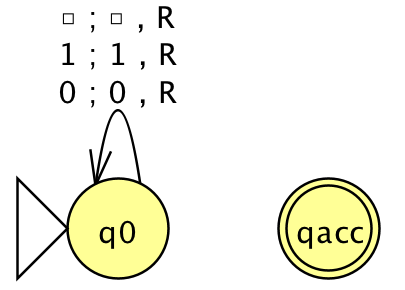
\includegraphics[width=1.5in]{Lect22TM1.png} ,  \varepsilon  \rangle$
    and  $M'$ is a Turing machine that computes like $M$ except, if the computation ever were to go to a  reject state,
    $M'$ loops instead.
    
    \vfill

    $F( \langle 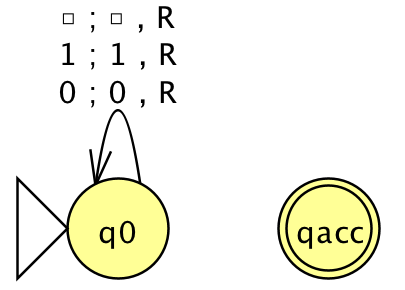
\includegraphics[width=1.5in]{Lect22TM1.png} ,  001  \rangle)$ =

    \vfill

    $F( \langle 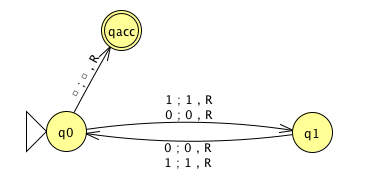
\includegraphics[width=2.5in]{Lect22TM2.png} ,  1  \rangle)$ =

    \vfill
    
    \newpage
    To use this function  to prove that $A_{TM} \leq_m HALT_{TM}$, we need  two claims:

    
    Claim (1): $F$ is computable \phantom{\hspace{2in}}
    
    \vfill

    Claim (2): for every  $x$,  $x \in  A_{TM}$ iff $F(x) \in HALT_{TM}$.  
    
    \vfill
     \vfill
\section*{Week10 monday}


Recall Definition  (Sipser 7.1): For  $M$ a deterministic decider, its {\bf running time} is the function  $f: \mathbb{N} \to \mathbb{N}$
given  by
\[
f(n) =  \text{max number of  steps $M$ takes before halting, over all inputs  of length $n$}
\]

Recall Definition (Sipser 7.7): For each function $t(n)$, the {\bf time complexity class}  $TIME(t(n))$, is defined  by
\[
TIME( t(n)) = \{ L \mid \text{$L$ is decidable by  a Turing machine with running time in  $O(t(n))$} \}
\]
Recall Definition (Sipser 7.12) : $P$ is the class of languages that  are decidable in polynomial time on 
a deterministic 1-tape  Turing  machine
\[
P  =  \bigcup_k TIME(n^k)
\]

Definition (Sipser  7.9): For $N$ a nodeterministic decider.  
The {\bf running time} of $N$ is the function $f: \mathbb{N} \to \mathbb{N}$ given  by
\[
f(n) =  \text{max number of  steps $N$ takes on  any branch before halting, over all inputs  of length $n$}
\]

Definition (Sipser 7.21): For each function $t(n)$, the {\bf nondeterministic time complexity class}  
$NTIME(t(n))$, is defined  by
\[
NTIME( t(n)) = \{ L \mid \text{$L$ is decidable by a nondeterministic Turing machine with running time in $O(t(n))$} \}
\]
\[
NP = \bigcup_k NTIME(n^k)
\]


{\bf True} or {\bf False}: $TIME(n^2) \subseteq NTIME(n^2)$

\vfill

{\bf True} or {\bf False}: $NTIME(n^2) \subseteq DTIME(n^2)$

\vfill
\newpage

{\bf Examples in $P$ }

{\it Can't use nondeterminism; Can use multiple tapes; Often need to be “more clever” than naïve / brute force approach}
\[
    PATH = \{\langle G,s,t\rangle \mid \textrm{$G$ is digraph with $n$ nodes there is path from s to t}\}
\]
Use breadth first search to show in $P$
\[
    RELPRIME = \{ \langle x,y\rangle \mid \textrm{$x$ and $y$ are relatively prime integers}\}
\]
Use Euclidean Algorithm to show in $P$
\[
    L(G) = \{w \mid \textrm{$w$ is generated by $G$}\} 
\]
(where $G$ is a context-free grammar). Use dynamic programming to show in $P$.

\vfill
{\bf Examples in $NP$}

{\it ``Verifiable" i.e. NP, Can be decided by a nondeterministic TM in polynomial time,
best known deterministic solution may be brute-force, 
solution can be verified by a deterministic TM in polynomial time.}

\[
    HAMPATH = \{\langle G,s,t \rangle \mid \textrm{$G$ is digraph with $n$ nodes, there is path
from $s$ to $t$ that goes through every node exactly once}\}
\]
\[
    VERTEX-COVER = \{ \langle G,k\rangle \mid \textrm{$G$ is an undirected graph with $n$
nodes that has a $k$-node vertex cover}\}
\]
\[
    CLIQUE = \{ \langle G,k\rangle \mid \textrm{$G$ is an undirected graph with $n$ nodes that has a $k$-clique}\}
\]
\[
    SAT =\{ \langle X \rangle \mid \textrm{$X$ is a satisfiable Boolean formula with $n$ variables}\}
\]

\vfill
\newpage
{\bf Every problem in NP is decidable with an exponential-time algorithm}

Nondeterministic approach: guess a possible solution, verify that it works.

Brute-force (worst-case exponential time) approach: iterate over all possible solutions, for each 
one, check if it works.



\begin{center}
\begin{tabular}{c|c}
    {\bf Problems in $P$} & {\bf Problems in $NP$}\\
    \hline
    (Membership in any) regular language & Any problem in $P$ \\
    (Membership in any) context-free language &  \\
    $A_{DFA}$ & $SAT$\\
    $E_{DFA}$ & $CLIQUE$ \\
    $EQ_{DFA}$ & $VERTEX-COVER$ \\
    $PATH$ & $HAMPATH$ \\
    $RELPRIME$ &  $\ldots$ \\
$\ldots$ &\\
\end{tabular}
\end{center}

Million-dollar question: Is $P = NP$?


One approach to trying to answer it is to look for {\it hardest} problems in $NP$ and 
then (1) if we can show that there are efficient algorithms for them, then we can get 
efficient algorithms for all problems in $NP$ so $P = NP$, or (2) these problems might 
be good candidates for showing that there are problems in $NP$ for which there 
are no efficient algorithms.

\vfill
\newpage
 \vfill
\section*{Week10 wednesday}



Definition (Sipser 7.29) Language  $A$ is {\bf polynomial-time mapping reducible} to language $B$, written $A \leq_P B$,
means there is a polynomial-time computable function $f: \Sigma^* \to \Sigma^*$  such that for every $x \in \Sigma^*$
\[
x \in A \qquad \text{iff} \qquad f(x) \in B.
\]
The  function $f$ is  called the  polynomial time reduction of $A$ to $B$.

{\bf  Theorem}  (Sipser 7.31):  If $A \leq_P B$ and $B  \in P$ then $A \in P$.

Proof: 

\vfill

Definition (Sipser 7.34; based in Stephen Cook and Leonid Levin's work in the 1970s): 
A language $B$ is {\bf  NP-complete} means (1) $B$ is in NP {\bf and}  (2) every language
$A$ in $NP$ is polynomial time reducible to $B$.

{\bf  Theorem}  (Sipser 7.35):  If $B$ is NP-complete and $B \in P$ then $P = NP$.

Proof: 

\vfill

\newpage

{\bf 3SAT}: A literal is a Boolean variable (e.g.  $x$) or a negated Boolean variable (e.g.  $\bar{x}$).  
A Boolean formula is a {\bf  3cnf-formula} if it is a Boolean formula in conjunctive normal form (a conjunction  
of  disjunctive clauses of literals) and each clause  has  three literals.
\[
3SAT  = \{  \langle  \phi \rangle \mid \text{$\phi$ is  a  satisfiable 3cnf-formula} \}
\]


Example strings  in $3SAT$
\vfill



Example  strings not  in $3SAT$

\vfill




{\bf Cook-Levin Theorem}: $3SAT$ is $NP$-complete.


{\it Are there other $NP$-complete problems?} To prove that $X$ is $NP$-complete
\begin{itemize}
\item {\it From scratch}: prove $X$ is in $NP$ and that all $NP$ problems are polynomial-time
reducible to $X$.
\item {\it Using reduction}: prove $X$ is in $NP$ and that a known-to-be $NP$-complete problem 
is polynomial-time reducible to $X$.
\end{itemize}

\vfill
\vfill


\newpage

{\bf CLIQUE}: A {\bf $k$-clique} in an undirected graph is a maximally connected subgraph with $k$  nodes.
\[
CLIQUE  = \{  \langle G, k \rangle \mid \text{$G$ is an  undirected graph with  a $k$-clique} \}
\]


Example strings  in $CLIQUE$

\vfill

Example  strings not  in $CLIQUE$

\vfill

Theorem (Sipser 7.32):
\[
3SAT  \leq_P CLIQUE
\]

Given a Boolean formula in conjunctive normal form with $k$ clauses and three literals per clause, we will 
map it to a graph so that the graph has a clique if the original formula is satisfiable and the 
graph does not have a clique if the original formula is not satisfiable.

The graph has $3k$ vertices (one for each literal in each clause) and an edge between all vertices except
\begin{itemize}
    \item vertices for two literals in the same clause
    \item vertices for literals that are negations of one another
\end{itemize}

Example: $(x \vee \bar{y} \vee {\bar z}) \wedge (\bar{x}  \vee y  \vee  z) \wedge (x \vee y  \vee z)$

\vfill

\newpage
 \vfill
\section*{Week10 friday}


\begin{center}
    \begin{tabular}{|p{4in}|p{3.5in}|}
        \hline
        & \\
        {\bf Model of Computation} & {\bf Class of Languages}\\
        &\\
        \hline
        & \\
        {\bf Deterministic finite automata}:
        formal definition, how to design for a given language, 
        how to describe language of a machine?
        {\bf Nondeterministic finite automata}:
        formal definition, how to design for a given language, 
        how to describe language of a machine?
        {\bf Regular expressions}: formal definition, how to design for a given language, 
        how to describe language of expression?
        {\it Also}: converting between different models. &
        {\bf Class of regular languages}: what are the closure 
        properties of this class? which languages are not in the class?
        using {\bf pumping lemma} to prove nonregularity.\\
        & \\
        \hline
        & \\
        {\bf Push-down automata}:
        formal definition, how to design for a given language, 
        how to describe language of a machine?
        {\bf Context-free grammars}:
        formal definition, how to design for a given language, 
        how to describe language of a grammar? &
        {\bf Class of context-free languages}: what are the closure 
        properties of this class? which languages are not in the class?\\
        & \\
        \hline
        & \\
        Turing machines that always halt in polynomial time
        & $P$ \\
        & \\
        Nondeterministic Turing machines that always halt in polynomial time 
        & $NP$ \\
        & \\
        \hline
        & \\
        {\bf Deciders} (Turing machines that always halt): 
        formal definition, how to design for a given language, 
        how to describe language of a machine? &
        {\bf Class of decidable languages}: what are the closure properties 
        of this class? which languages are not in the class? using diagonalization
        and mapping reduction to show undecidability \\
        & \\
        \hline
        & \\
        {\bf Turing machines}
        formal definition, how to design for a given language, 
        how to describe language of a machine? &
        {\bf Class of recognizable languages}: what are the closure properties 
        of this class? which languages are not in the class? using closure
        and mapping reduction to show unrecognizability \\
        & \\
        \hline
    \end{tabular}
\end{center}

\newpage

{\bf Given a language, prove it is regular}

{\it Strategy 1}: construct DFA recognizing the language and prove it works.

{\it Strategy 2}: construct NFA recognizing the language and prove it works.

{\it Strategy 3}: construct regular expression recognizing the language and prove it works.

{\it ``Prove it works'' means \ldots}

\vspace{100pt}

{\bf Example}: $L  = \{ w \in \{0,1\}^* \mid \textrm{$w$ has odd number of $1$s or starts with $0$}\}$

Using NFA

\vfill

Using regular expressions

\vfill


\newpage

{\bf Example}: Select all and only the options that result in a true statement: ``To show 
a language $A$ is not regular, we can\ldots'' 

\begin{enumerate}
    \item[a.] Show $A$ is finite
    \item[b.] Show there is a CFG generating $A$
    \item[c.] Show $A$ has no pumping length
    \item[d.] Show $A$ is undecidable
\end{enumerate}

\newpage

{\bf Example}: What is the language generated by the CFG with rules
\begin{align*}
    S &\to aSb \mid bY \mid Ya \\
    Y &\to bY \mid Ya \mid \varepsilon 
\end{align*}

\newpage

{\bf Example}: Prove that the language 
$T = \{ \langle M \rangle \mid \textrm{$M$ is a Turing machine and $L(M)$ is infinite}\}$ 
is undecidable.

\newpage

{\bf Example}: Prove that the class of decidable languages is closed under concatenation.
 \vfill
\end{document}